\chapter{State of the Art} 
\label{chap:Chapter2}
%-------------------------------------------------------------------------------%
\section{UAV}
TODO: MORE INFO\\
TODO: ADD FIGURES

\subsection{Propeller Fundamentals}
The purpose of a propeller is to convert the rotational power produced by the engine into forward thrust during flight.
This is achieved by accelerating a mass of air through the blades of the propeller as it spins, generating the necessary force to propel the aircraft forward at a specific airspeed \cite{main_uav}.
Figure \ref{fig:propeller}, illustrates the connection between the changing the propeller rotation speed and the speed and movement.

\begin{figure}[H]
    \centering
    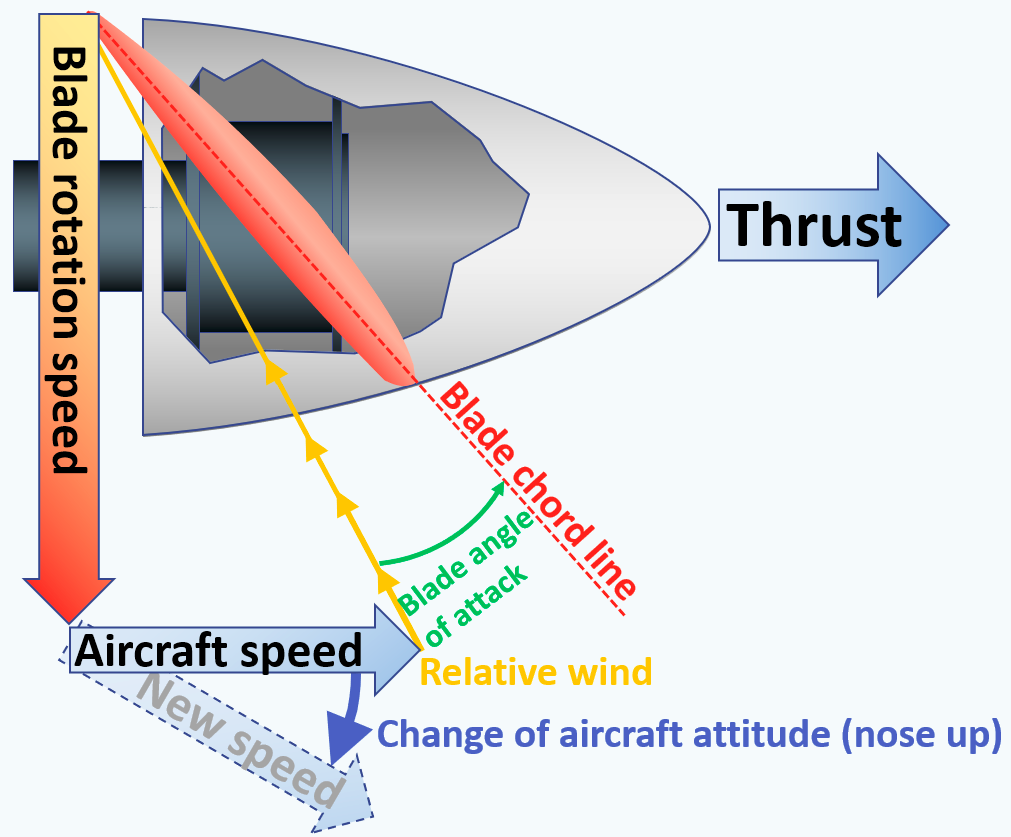
\includegraphics[scale=0.25]{ch2/assets/propeller.png}
    \caption{Propeller blade representation \cite{propeller}}
    \label{fig:propeller}
\end{figure}

The propeller performance can be affected by \cite{main_uav}:
\begin{itemize}
    \item Blade diameter
    \item Number of blades
    \item Blade pitch
\end{itemize}

The propeller diameter is often desired as high as the motor can support.
High diameter helps for hover mode for better hover lift efficiency but airplane mode at high speeds can be very inefficient.
The higher the diameter, the higher the inertia and the higher the tip speed[23].
When tip speed reaches near sonic levels, the potential to have a windmill effect occurs, to avoid that, the disc diameter must be study for limitations as airspeed increases through the blade.

The number of blades affects the thrust and efficiency.
Hence, considering thrust per number of blades, generally the fewer blades design result in more efficient propeller disc [23].
Generally, small UAV applications using a two-blade configuration is a good compromise of thrust and efficiency.
However, increasing the number of blades is the best solution to efficiently extract the desired thrust from a motor where a propeller with fewer blades cannot reach the required thrust for operation and in cases where vibration and noise are also an issue.

The propeller pitch refers to the distance that the propeller advances through the air during one revolution.
A fine pitch means it will move forward through the air a short distance every revolution (low advance ratio) whereas a coarse pitch moves forward through the air a large distance every revolution (high advance ratio)[23].
Thus for hover mode, a fine pitch is recommended.
But for airplane mode when in cruise operation due to high speeds a coarse pitch is the most efficient configuration.
In climb operation a pitch higher than the fine pitch for take-off but less coarse pitch than the cruise is required.

\subsection{Fixed Pitch Proprotors}
TODO: MORE INFO\\
TODO: ADD FIGURES

\subsection{Variable Pitch Proprotors}
Historically, early aviation pioneers experimented with propellers that could only be adjusted on the ground.
The first automatic variable pitch air screw was patented by L. E. Baines in 1919.
The Gloster Hele-Shaw Beacham variable pitch propeller, developed in 1928, demonstrated practical controllable pitch capabilities.
Over time, various designs and mechanisms, including hydraulic and pneumatic systems, were explored and refined.
The development of constant-speed propellers marked a significant advancement in aviation technology, offering improved efficiency and performance \cite{VPP2}.\\

A significant advantage of variable-pitch propellers is their ability to adapt to varying airspeeds. 
When an aircraft is stationary or moving slowly, the propeller blades can be set to a low angle of attack to reduce drag. As the aircraft gains speed, the pitch is increased to maintain optimal performance. 
This adaptability ensures efficient operation across a range of flight conditions.

The primary purpose of variable pitch propellers is to maintain the optimal angle of attack relative to the changing wind vector as the aircraft accelerates.
Traditional fixed-pitch propellers face efficiency challenges in various flight conditions.
Adjustable blade angles address this issue, allowing for improved efficiency during takeoff, climb, and cruise.\cite{VPP3}.\\

Variable-pitch systems can adjust blade pitch to maintain a selected \gls{RPM} enhancing overall performance, especially at high altitudes, by allowing the rotor to operate in its most economical speed range \cite{VPP2}, \cite{VPP3}.\\

Three methods change the pitch: Hydraulic, Centrifugal, and Electromechanical control \cite{VPP2}.\\
TODO: ADD FIGURES

\subsubsection{Hydraulic Method}
This system involves the use of engine oil pressure to control the pitch-changing mechanism and consists of a pump, control valves, and cylinders that actuate the movement of the propeller blades.
In an aircraft without a variable-pitch proprotor system, the pilot uses hydraulics to manually control the pitch of the propeller blades \cite{VPP2}.\\

Hydraulic systems provide a precise means of adjusting the propeller pitch, allowing efficient performance under different flight conditions, and contributing to the overall safety and reliability of the system.\\

But Hydraulic systems add complexity and weight to the overall aircraft system. 
More components means more elements could potentially fail or require maintenance. 
There is also the risk of fluid leakage or fluid contamination that may lead to a reduction in hydraulic pressure, potentially affecting the pitch control mechanism.
Hydraulic systems may have a slow response time due to the time it takes for hydraulic pressure changes to propagate through the system which might be a concern in situations where rapid adjustments are required.\cite{VPP2}
TODO: ADD FIGURES

\subsubsection{Centrifugal Method}
In the centrifugal systems, centrifugal weights can be attached directly to the propellers.
An eccentric weight is placed near or in the spinner and secured with a spring and, when the propeller reaches a certain \gls{RPM}, centrifugal force swings the weights outward, driving a mechanism that twists the propeller to a steeper pitch. 
As the propeller slows down, the \gls{RPM} drops and the spring pushes the weight back, readjusting the propeller pitch to a shallower pitch.

As advantages, centrifugal systems are simpler compared to hydraulic systems since they involve fewer components.
The reliance on mechanical components driven by centrifugal force can enhance reliability because there are fewer points of failure.
There is no need to use external power sources, such as an engine-driven pump.
Also, centrifugal systems can operate automatically without direct pilot intervention.
The system responds to changes in rotational speed without the need for continuous manual control.

However, centrifugal systems may provide less precise pitch control than more advanced hydraulic or electronic systems. This limitation can affect the ability to finely tune the propeller for optimal performance.
The response time of centrifugal systems may be slower compared to more sophisticated systems. This limitation could be a factor in situations where rapid adjustments to the propeller pitch are necessary.\cite{VPP2}

TODO: ADD FIGURES

\subsubsection{Electromechanical Method}
These systems involve electric motors and mechanical linkages to control the pitch of the propeller blades.\\

Electromechanical methods provide precise control over the pitch of the propeller blades, can offer rapid response times to changes in flight conditions, are often versatile, and can be adapted for various aircraft configurations.
Compared to certain hydraulic systems, electromechanical systems might require less maintenance.
They often have fewer components prone to wear and can be more straightforward to service.\\

As disadvantages, electromechanical systems, including motors and associated components, can add weight to the aircraft, require electrical power to operate, and are more complex than purely mechanical systems, increasing the chance of failures.\cite{VPP2}

TODO: ADD FIGURES
\href{https://www.youtube.com/watch?v=MpsBOQOUB-4}{\textit{VPP Video}}
%-------------------------------------------------------------------------------%
